\documentclass[11pt]{article}
	
%%%%%%%%%%%%%%%%%%%%%%%%%%%%%%%%%%%%%%%%%%%%%%%%%%%%%%%%%%%%%%%%%%%%%%
%\pdfminorversion=4
% NOTE: To produce blinded version, replace "0" with "1" below.
\newcommand{\blind}{0}

%%%%%%% IISE Transactions margin specifications %%%%%%%%%%%%%%%%%%%
% DON'T change margins - should be 1 inch all around.
\addtolength{\oddsidemargin}{-.5in}%
\addtolength{\evensidemargin}{-.5in}%
\addtolength{\textwidth}{1in}%
\addtolength{\textheight}{1.3in}%
\addtolength{\topmargin}{-.8in}%
\makeatletter
\renewcommand\section{\@startsection {section}{1}{\z@}%
                                   {-3.5ex \@plus -1ex \@minus -.2ex}%
                                   {2.3ex \@plus.2ex}%
                                   {\normalfont\fontfamily{phv}\fontsize{16}{19}\bfseries}}
\renewcommand\subsection{\@startsection{subsection}{2}{\z@}%
                                     {-3.25ex\@plus -1ex \@minus -.2ex}%
                                     {1.5ex \@plus .2ex}%
                                     {\normalfont\fontfamily{phv}\fontsize{14}{17}\bfseries}}
\renewcommand\subsubsection{\@startsection{subsubsection}{3}{\z@}%
                                    {-3.25ex\@plus -1ex \@minus -.2ex}%
                                     {1.5ex \@plus .2ex}%
                                     {\normalfont\normalsize\fontfamily{phv}\fontsize{14}{17}\selectfont}}
\makeatother
%%%%%%%%%%%%%%%%%%%%%%%%%%%%%%%%%%%%%%%%%%%%%%%%%%%%%%%%%%%%%%%%%%%%%%%%%

%%%%% IISE Transactions package list %%%%%%%%%%%%%%%%%%%%%%%%%%%%%%%%%%%%%%
\usepackage{amsmath}
\usepackage{graphicx}
\usepackage{enumerate}
\usepackage{natbib} %comment out if you do not have the package
\usepackage{url} % not crucial - just used below for the URL
%%%%%%%%%%%%%%%%%%%%%%%%%%%%%%%%%%%%%%%%%%%%%%%%%%%%%%%%%%%%%%%%%%%%%%%

%%%%% Author package list and commands %%%%%%%%%%%%%%%%%%%%%%%%%%%%%%%%%%%%%%%%%%%%%
%%%%% Here are some examples %%%%%%%%%%%%%%
%	\usepackage{amsfonts, amsthm, latexsym, amssymb}
%	\usepackage{lineno}
%	\newcommand{\mb}{\mathbf}
%%%%%%%%%%%%%%%%%%%%%%%%%%%%%%%%%%%%%%%%%%%%%%%%%%%%%%%%%%%%%%%%%%%%%%%%%%%%%%

\begin{document}
	
		%%%%%%%%%%%%%%%%%%%%%%%%%%%%%%%%%%%%%%%%%%%%%%%%%%%%%%%%%%%%%%%%%%%%%%%%%%%%%%
	\def\spacingset#1{\renewcommand{\baselinestretch}%
		{#1}\small\normalsize} \spacingset{1}
	%%%%%%%%%%%%%%%%%%%%%%%%%%%%%%%%%%%%%%%%%%%%%%%%%%%%%%%%%%%%%%%%%%%%%%%%%%%%%%
	
	\if0\blind
	{
		\title{\bf Simulation-guided Data Assimilation for Kinetics Modeling of Potassium Channel Isoforms in Mouse Cardiomyocytes}
		\author{Haedong Kim $^a$, Hui Yang $^a$, Andrew R. Ednie $^b$, and Eric S. Bennett $^b$ \\
		$^a$ Department of Industrial and Manufacturing Engineering, \\
		The Pennsylvania State University, State College, PA USA \\
        $^b$ Department of Neuroscience, Cell Biology, and Physiology, \\
        Wright State University, City, OH USA}
		\date{}
		\maketitle
	} \fi
	
	\if1\blind
	{
        \title{\bf \emph{IISE Transactions} \LaTeX \ Template}
		\author{Author information is purposely removed for double-blind review}
		
\bigskip
		\bigskip
		\bigskip
		\begin{center}
			{\LARGE\bf \emph{IISE Transactions} \LaTeX \ Template}
		\end{center}
		\medskip
	} \fi
	\bigskip
		
\begin{abstract}
This document provides a \LaTeX \ template for \emph{IISE Transactions}. Your paper should be compiled in the following order: title; abstract; keywords; main text, including an introduction and a conclusion or summary; acknowledgments; declaration of interest statement; references; appendices (as appropriate). Figures and tables should be inserted into the text as close to first mention as possible (NOT appended to the end of the manuscript). In-text citations and the reference list must follow \emph{IISE Transactions} guidelines. Use 11 point font, 1 inch margins, and double-spacing for the manuscript. A typical paper for this journal should be no more than 30 pages in manuscript format, counting from the title page to references. Appendices should be included as supplemental online materials. Do not use footnotes. \emph{IISE Transactions} uses a double-blind review process. Please make sure that you submit the \textbf{blind version} of your manuscript, which does not contain any information identifying the authors.  This includes removing the authors information on the title page as well as the information that may be identifying in the Acknowledgment section. We thank you for your attention to these details.
\end{abstract}
		
\noindent%
{\it Keywords:} \emph{IISE Transactions}; \LaTeX; Manuscript format; Taylor \& Francis.

%\newpage
\spacingset{1.5} % DON'T change the spacing!


\section{Introduction} \label{s:intro}
\begin{itemize}
    \item \textbf{Motivation} Voltage-gated ion channels (VGICs) are the functional unit of the electrical conduction system of the heart that controls the synchronous contraction of numerous cardiomyocytes. Among major cardiac VGICs, K\textsuperscript{+} channels (K\textsubscript{v}) have a distinctive feature: they have various isoforms that contribute to K\textsuperscript{+} current, while the dominant isoform is responsible for Na\textsuperscript{+} and Ca\textsuperscript{2+} currents. Although each K\textsubscript{+} generated through K\textsubscript{v} isoform has a different role in the repolarization phase, only the sum of these individual K\textsuperscript{+} currents (I\textsubscript{Ksum}) can be recorded through in-vitro experiments. Data analysis tools are used to estimate information about K\textsubscript{v} isoforms from experimental I\textsubscript{Ksum} recordings.
    \item \textbf{Gaps \& Needs} A traditional approach is based on the data-driven curve fitting method that assumes the functional forms for the shape of individual K\textsuperscript{+} currents. This method directly fits individual K\textsuperscript{+} currents to experimental I\textsubscript{Ksum} recordings by searching the shape parameters of the current functions that have the best fit. It has been proven that the curve fitting approach describes I\textsubscript{Ksum} well with estimated K\textsuperscript{+} currents. However, the mathematical form of this classical method only characterizes the shape of the currents, not the kinetics of corresponding K\textsubscript{v} isoforms. In addition, the curve fitting method handles experimental I\textsubscript{Ksum} recordings from the same cell independently, so it lacks the cellular-level analysis.
    \item \textbf{Objective} As opposed to the traditional data-driven curve fitting method, we propose a novel framework of biophysics-driven data assimilation method for kinetics modeling of K\textsubscript{v} isoforms based on computer models of K\textsuperscript{+} currents that can simulate underlying gating kinetics of the currents.
    \item \textbf{Approach} 
    \item \textbf{Experiment \& Performance} The proposed framework outperforms the curve fitting method for minimizing discrepancies between experimental and estimated total K\textsuperscript{+} currents. We also provide the kinetics modeling results that are not possible in the traditional method.
    \item \textbf{Significance} Experimental results show that the proposed method has strong potential to be a novel analysis tool to decompose I\textsubscript{Ksum} recordings to estimate not only the current characteristics but also kinetics of K\textsubscript{v} isoforms.
\end{itemize}

The review of literature can be a separate section but it can be merged with the introduction section. One can find a number of reference examples at the end of this template, like,
\begin{itemize}
\item A book: \cite{Hastie2009}.
\item A journal article: \cite{Byon2013}.
\item A conference paper: \cite{Breunig2000}.
\item A book chapter: \cite{Yang2010}.
\item A technical report: \cite{Kelley2007}.
\end{itemize}

\section{Methods} \label{s:methods}

\subsection{\emph{Computer Models of Potassium Channel Isoforms}} \label{s:methods.1}
modeling (mathematical equations)
\begin{figure}
    \centering
    \includegraphics{figs/ap_underlying_currents.pdf}
    \caption{Caption}
    \label{fig:ap_underlying_currents}
\end{figure}

\subsection{\emph{Sensitivity Analysis of Calibration Parameters}} \label{s:methods.2}
this section shows the results of the variable screening.
\begin{figure}
    \centering
    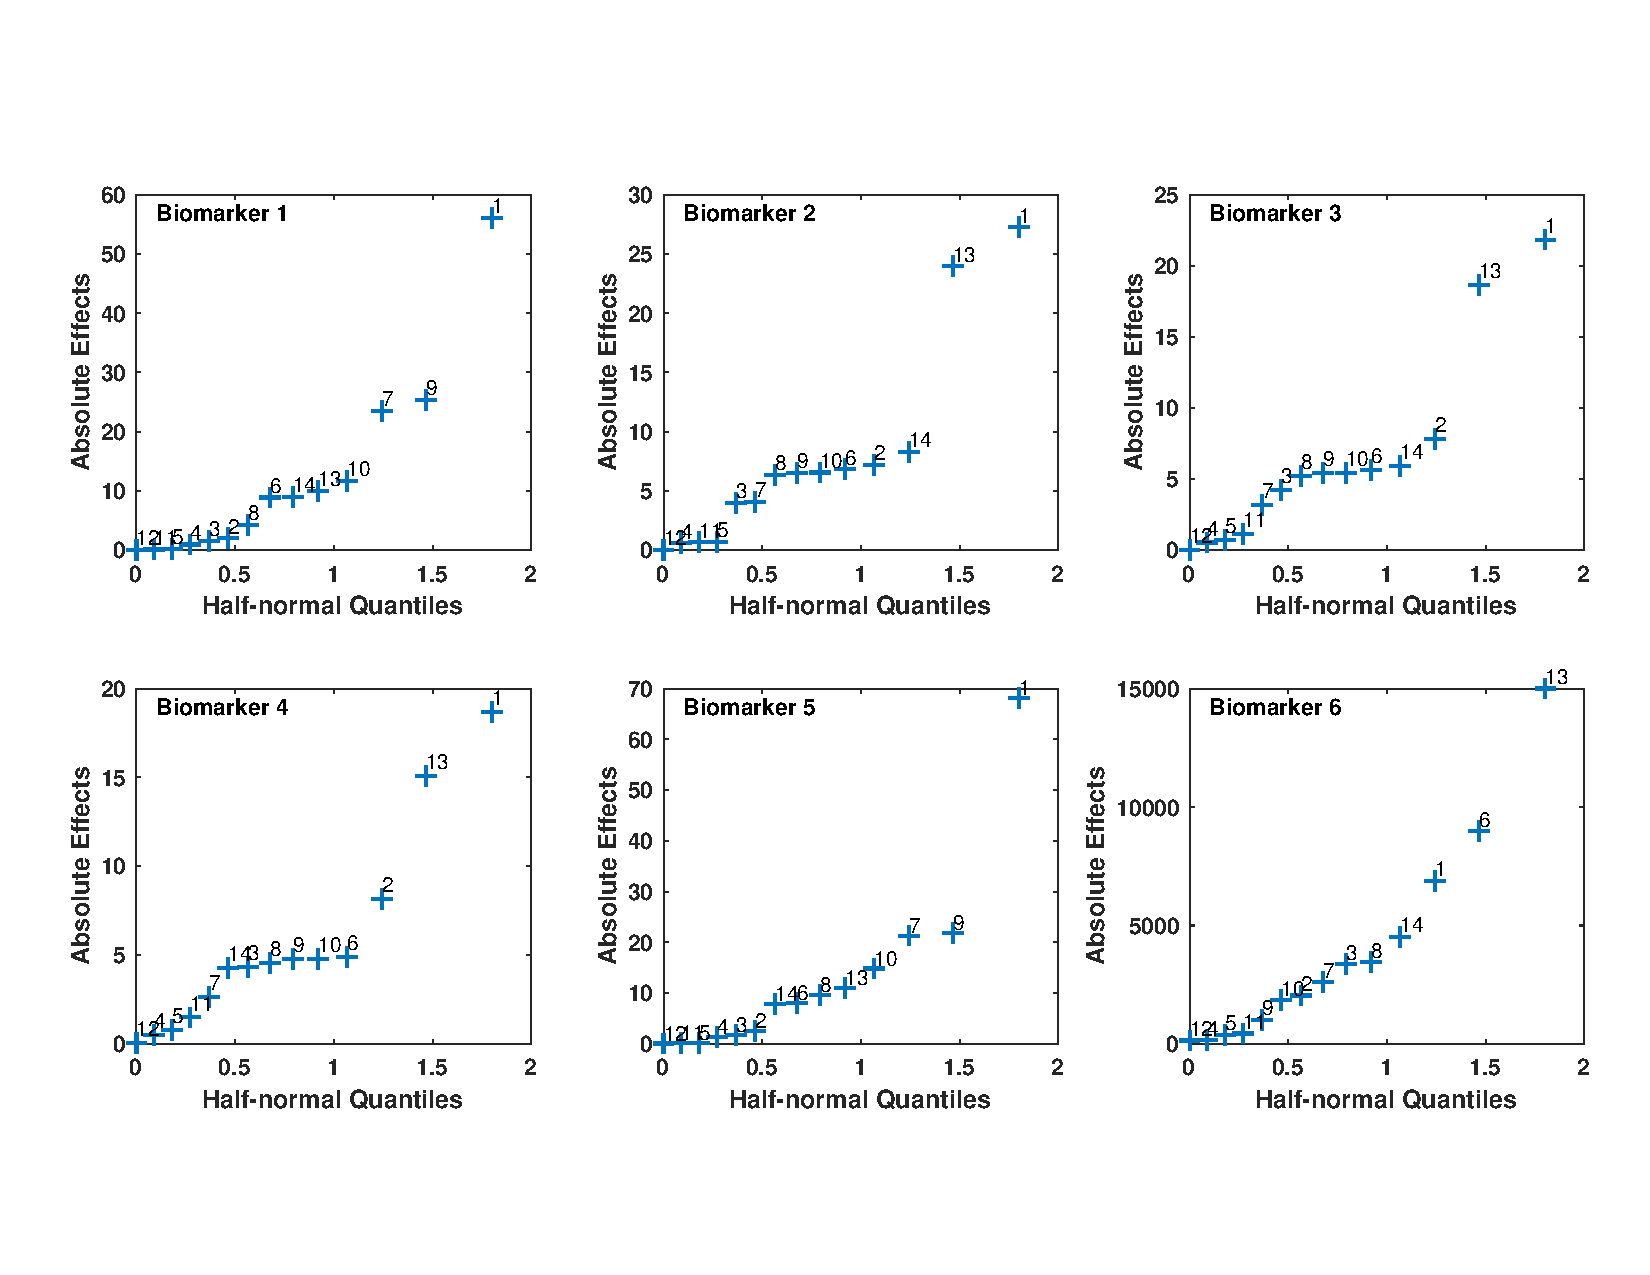
\includegraphics{figs/doe_kto.pdf}
    \caption{Half-normal plots I\textsubscript{Kto}}
    \label{fig:doe_kto}
\end{figure}

\begin{figure}
    \centering
    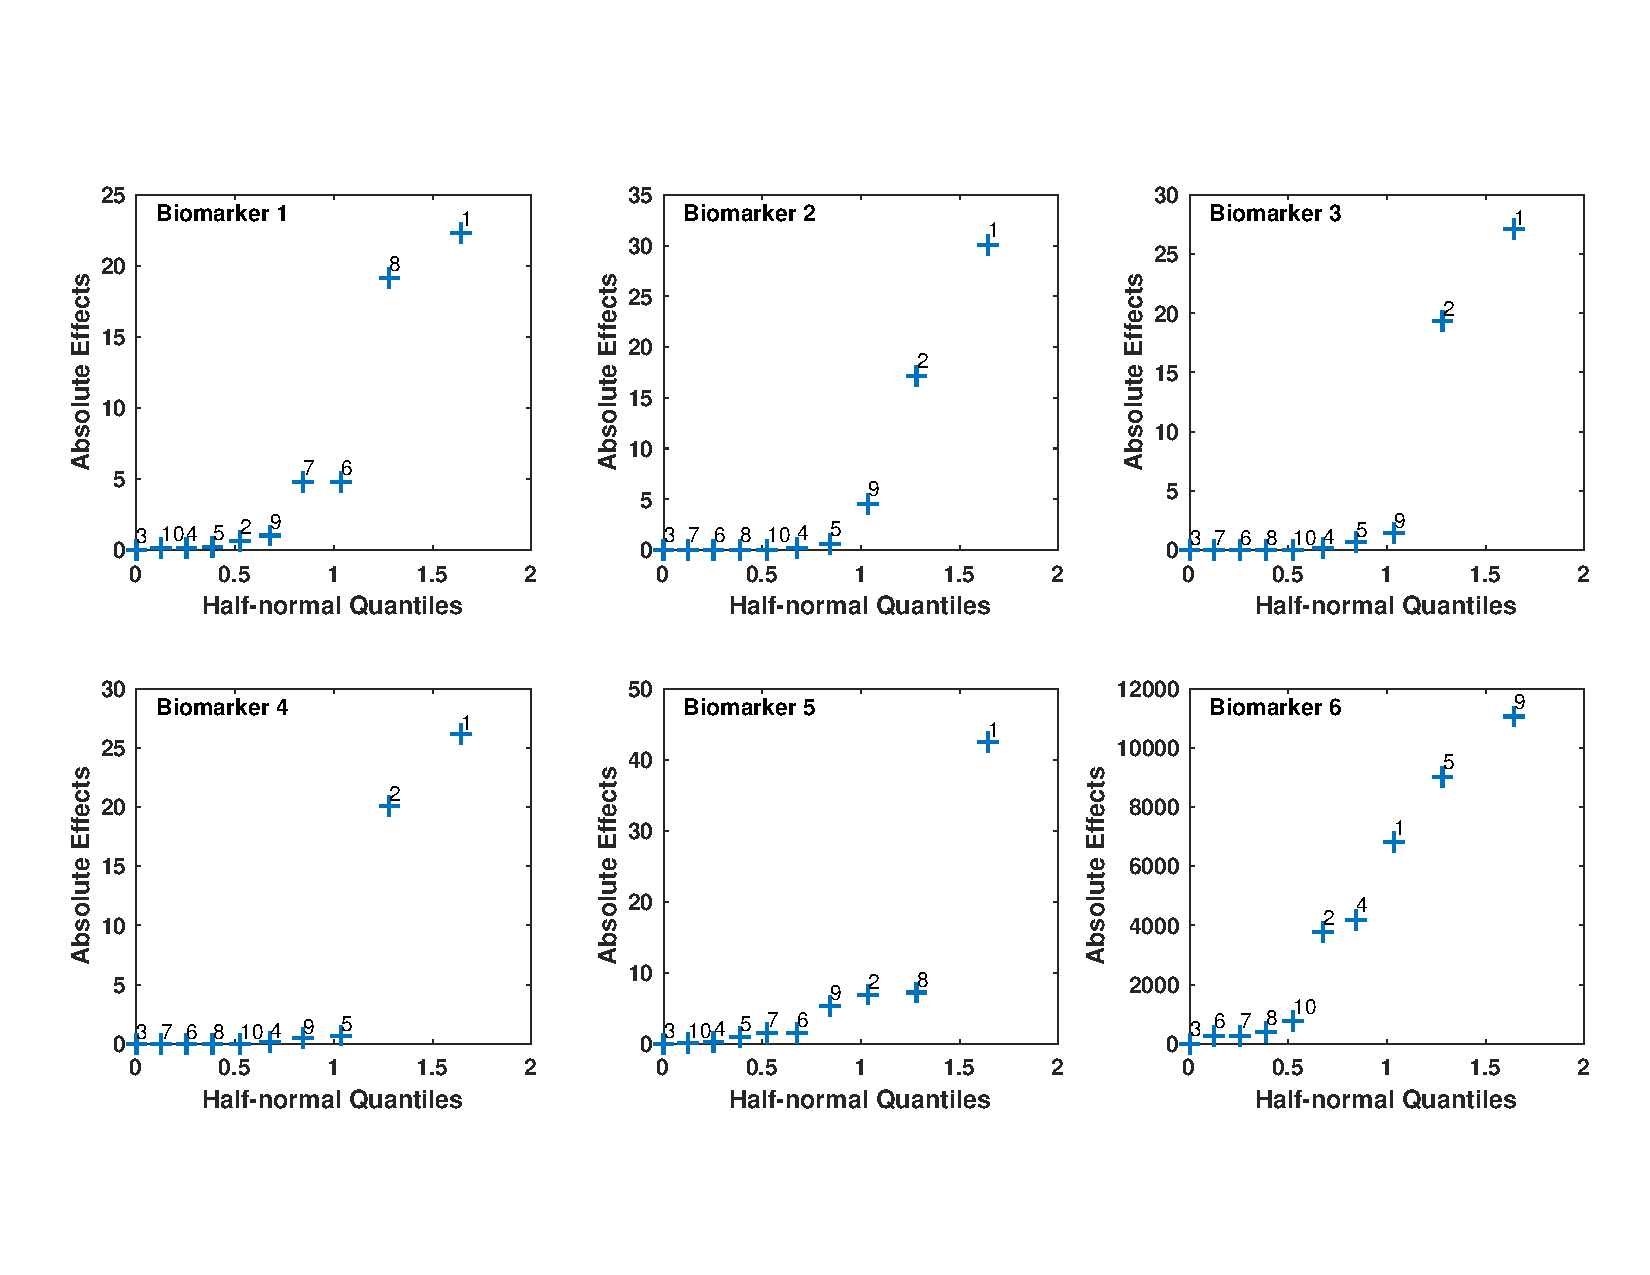
\includegraphics{figs/doe_kslow1.pdf}
    \caption{Half-normal plots I\textsubscript{Kslow1}}
    \label{fig:doe_kslow1}
\end{figure}

\begin{figure}
    \centering
    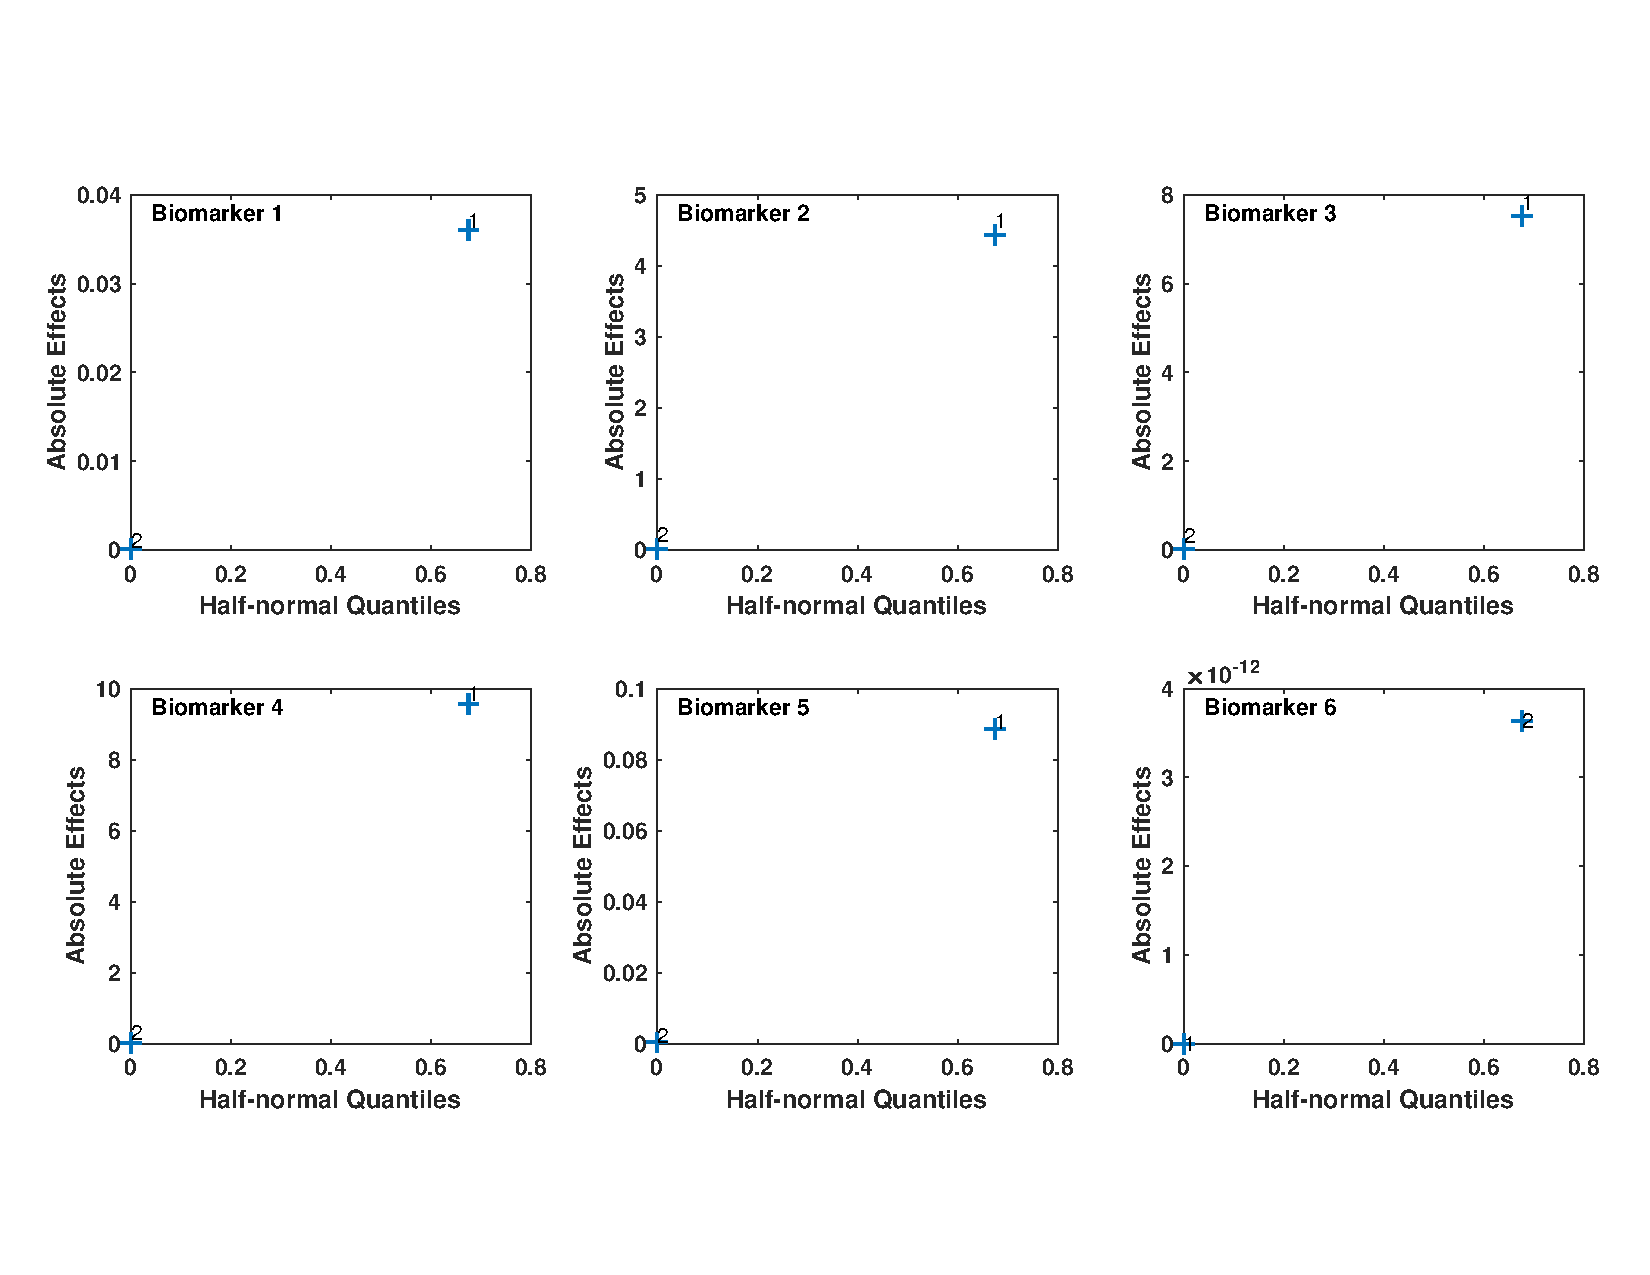
\includegraphics{figs/doe_kslow2.pdf}
    \caption{Half-normal plots I\textsubscript{Kslow2}}
    \label{fig:doe_kslow2}
\end{figure}

\begin{figure}
    \centering
    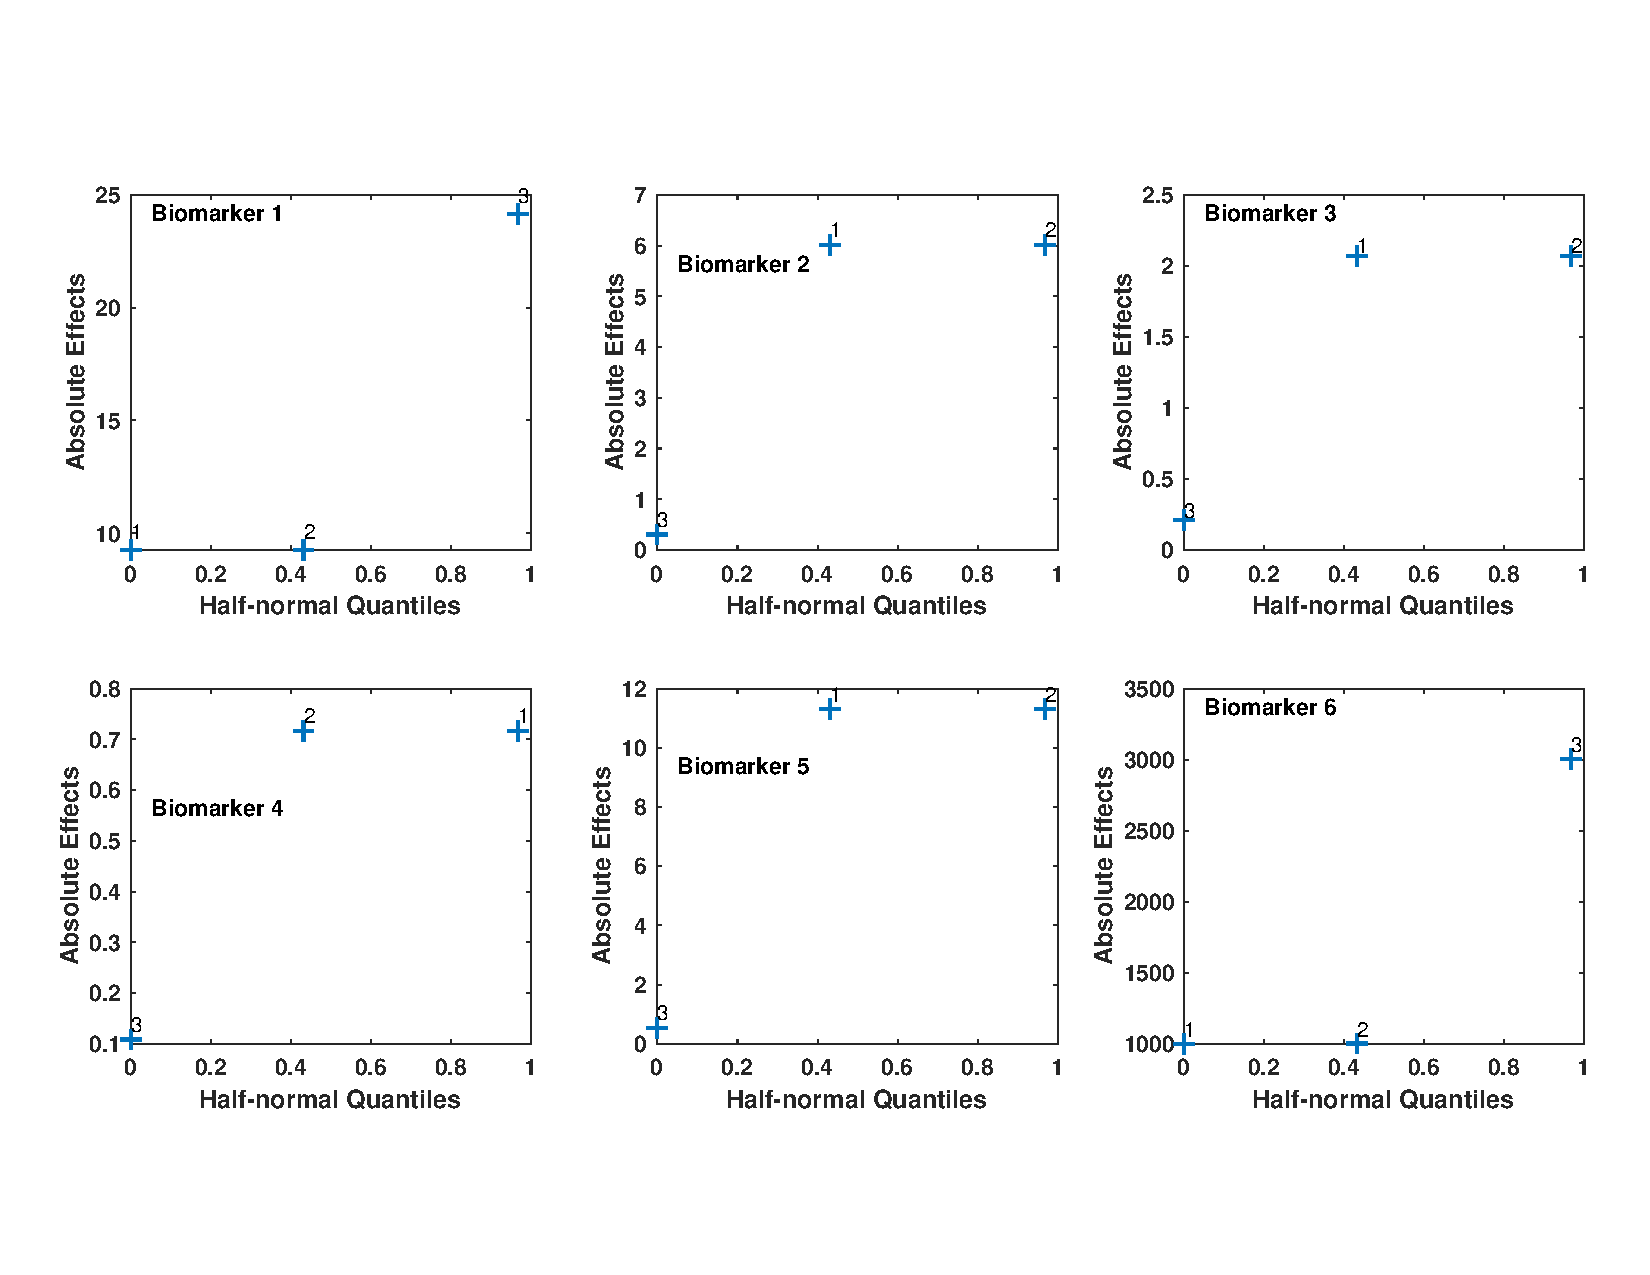
\includegraphics{figs/doe_kss.pdf}
    \caption{Half-normal plots I\textsubscript{Kss}}
    \label{fig:doe_kss}
\end{figure}

\subsection{\emph{Model Calibration}} \label{s:methods.3}
calibration procedure; non-linear optimization methods

\subsection{\emph{Graphical User Interface}} \label{s:methods.4}
show how to use it

\subsection{\emph{Case Study Glycosylations}} \label{s:methods.5}
case study

\section{Results} \label{s:results}
Perhaps numerical analysis of performance, comparison, and demonstration of applicability and impact using real data.

\section{Conclusion}\label{s:conclusion}
A paper ends with a conclusion or summary section.

\if0\blind{
\section*{Acknowledgements}
The authors acknowledge the generous support from the funding agency of XYZ.	} \fi

\bibliographystyle{chicago}
\spacingset{1}
\bibliography{IISE-Trans}
	
\end{document}
